\documentclass{article}

\usepackage[utf8]{inputenc}
\usepackage{enumitem}
\usepackage{todonotes}
\usepackage[ngerman]{babel}
\usepackage{amsmath}
\usepackage{float}
\usepackage{pgfplots}

% Roman numerals: \rom{123}
\makeatletter
\newcommand*{\rom}[1]{\expandafter\@slowromancap\romannumeral #1@}
\makeatother

\newcommand{\sig}{\text{sig}}
\newcommand{\relu}{\text{ReLU}}
\newcommand{\leakyrelu}{\text{Leaky-ReLU}}
\newcommand{\elu}{\text{ELU}}
\newcommand{\selu}{\text{SELU}}

\renewcommand{\exp}[1]{\text{exp}\big(#1\big)}

\title{Blatt 10}
\author{Luca Krüger, Jonas Otto, Jonas Merkle (Gruppe R)}
\date{\today}

\begin{document}
\maketitle
\section{Transferfunktionen}

\begin{enumerate}
\item 
\begin{enumerate}[label=\alph*)]
\item
\begin{align*}
\text{zz: } \text{sig}(x) &= \frac{1+ \tanh{\frac{x}{2}}}{2} \\ \\
&=\frac{1}{2} \Bigg(1+ \frac{\exp{\frac{x}{2}} - \exp{\frac{-x}{2}}}{\exp{\frac{x}{2}}+\exp{-\frac{x}{2}}}\Bigg)\\
&=\frac{1}{2}\Bigg(\frac{\exp{\frac{x}{2}}+\exp{\frac{-x}{2}}+\exp{\frac{x}{2}}-\exp{\frac{-x}{2}}}{\exp{\frac{x}{2}}+\exp{\frac{-x}{2}}}\Bigg)\\
&=\frac{1}{2} \Bigg(\frac{2\exp{\frac{x}{2}}}{\exp{\frac{x}{2}}+\exp{\frac{-x}{2}}}\Bigg) =\frac{\exp{\frac{x}{2}}}{\exp{\frac{x}{2}}+\exp{\frac{-x}{2}}}\\
&=\frac{1}{1+ \exp{\frac{-x}{2}+\frac{-x}{2}}} \\
&= \frac{1}{1+e^{-x}} 
\end{align*}
\item
Vorzeichen der Gewichte:
\begin{figure}[H]
  \centering
  \tikzstyle{inputNode}=[draw,circle,minimum size=10pt,inner sep=0pt]
  \tikzstyle{stateTransition}=[->, thick]
  \begin{tikzpicture}

\node[draw,circle,minimum size=40pt,inner sep=0pt] (s11) at (0,3) {$\tanh(x)$};
\node[draw,circle,minimum size=40pt,inner sep=0pt] (s12) at (0,1) {$\tanh(x)$};
\node[draw,circle,minimum size=40pt,inner sep=0pt] (s13) at (0,-1){$\tanh(x)$};
\node[draw,circle,minimum size=40pt,inner sep=0pt] (s14) at (0,-3){$\tanh(x)$};
\node[draw,circle,minimum size=40pt,inner sep=0pt] (s21) at (3,1) {$\tanh(x)$};
\node[draw,circle,minimum size=40pt,inner sep=0pt] (s22) at (3,-1){$\tanh(x)$};


    \draw[stateTransition,red] (s11) to[] node [pos=.7,above=5pt] {} (s21);
    \draw[stateTransition,blue] (s11) to[] node [pos=.7,above=5pt] {} (s22);
    \draw[stateTransition,red] (s12) to[] node [pos=.7,above=5pt] {} (s21);
    \draw[stateTransition,blue] (s12) to[] node [pos=.7,above=5pt] {} (s22);
    \draw[stateTransition,blue] (s13) to[] node [pos=.7,above=5pt] {} (s21);
    \draw[stateTransition,red] (s13) to[] node [pos=.7,above=5pt] {} (s22);
    \draw[stateTransition,blue] (s14) to[] node [pos=.7,above=5pt] {} (s21);
    \draw[stateTransition,red] (s14) to[] node [pos=.7,above=5pt] {} (s22);
    \begin{axis}[%
    hide axis,
    xmin=10,
    xmax=50,
    ymin=0,
    ymax=0.4,
    legend style={draw=white!15!black,legend cell align=left}
    ]
    \addlegendimage{red}
    \addlegendentry{$w>0$};
    \addlegendimage{blue}
    \addlegendentry{$w<0$};
    \end{axis}
  \end{tikzpicture}
  \caption{Tanh-Neuronen}
\end{figure}
\begin{figure}[H]
  \centering
  \tikzstyle{inputNode}=[draw,circle,minimum size=10pt,inner sep=0pt]
  \tikzstyle{stateTransition}=[->, thick]
  \begin{tikzpicture}

\node[draw,circle,minimum size=40pt,inner sep=0pt] (s11) at (0,3)  {$\sig(x)$};
\node[draw,circle,minimum size=40pt,inner sep=0pt] (s12) at (0,1)  {$\sig(x)$};
\node[draw,circle,minimum size=40pt,inner sep=0pt] (s13) at (0,-1) {$\sig(x)$};
\node[draw,circle,minimum size=40pt,inner sep=0pt] (s14) at (0,-3) {$\sig(x)$};
\node[draw,circle,minimum size=40pt,inner sep=0pt] (s21) at (3,1)  {$\sig(x)$};
\node[draw,circle,minimum size=40pt,inner sep=0pt] (s22) at (3,-1) {$\sig(x)$};


    \draw[stateTransition,red] (s11) to[] node [pos=.7,above=5pt] {} (s21);
    \draw[stateTransition,blue] (s11) to[] node [pos=.7,above=5pt] {} (s22);
    \draw[stateTransition,red] (s12) to[] node [pos=.7,above=5pt] {} (s21);
    \draw[stateTransition,blue] (s12) to[] node [pos=.7,above=5pt] {} (s22);
    \draw[stateTransition,red] (s13) to[] node [pos=.7,above=5pt] {} (s21);
    \draw[stateTransition,blue] (s13) to[] node [pos=.7,above=5pt] {} (s22);
    \draw[stateTransition,red] (s14) to[] node [pos=.7,above=5pt] {} (s21);
    \draw[stateTransition,blue] (s14) to[] node [pos=.7,above=5pt] {} (s22);
    \begin{axis}[%
    hide axis,
    xmin=10,
    xmax=50,
    ymin=0,
    ymax=0.4,
    legend style={draw=white!15!black,legend cell align=left}
    ]
    \addlegendimage{red}
    \addlegendentry{$w>0$};
    \addlegendimage{blue}
    \addlegendentry{$w<0$};
    \end{axis}
  \end{tikzpicture}
  \caption{Sigmoid-Neuronen}
\end{figure}
\end{enumerate}
\item
\begin{enumerate}[label=\alph*)]
\item
Unter der Verwendung von \textit{Rectified Linear Units} ist für dentritische Potential $u<0$ die Ausgabe des Neurons $y=0$ sowie der Gradient $\frac{\partial E}{\partial w}=0$. Dadurch kommt es bei dem Neuron zu einem \textit{Learning Slowdown}. Dieses Verhalten propagiert sich außerdem durch vorhergehende Schichten im Netzwerk. Für $u>0$ ist der Gradient konstant.
\item
$\tanh(x)$ erfordert aufgrund der komplexen Berechnung von Winkelfunktionen einen hohen Rechenaufwand.
Die Performance des Lernvorgang ist daher wahrscheinlich erheblich besser, wenn eine weniger komplexe Funktion wie $\text{ReLU}(x)$ verwendet wird.
\item
Für $u_i<0$ gilt:
\begin{align*}
\relu(u_i)=y_i^{(1)}=0 \ \Rightarrow \ \frac{\partial E}{\partial w_{ij}^{(2)}}=\delta_j^{(2)} f'(u_j^{(2)}) y_i^{(2)}=0 \\
\end{align*}
In der Regel ist der rückwärts propagierte Fehler $\delta_i^{(k)} \propto f'(u_i^{(k+1)})$, wonach in unserem Fall ($u_i<0$) und $\relu'(u_i^{(k+1)})=0$ auch Lernschritte vorheriger Neuronen blockiert werden.\\
Für $\leakyrelu(x)$ als Transferfunktion treten diese Probleme nicht auf, da für den Fall $u_i<0$ gilt:
\begin{align*}
\leakyrelu(u_i) \neq 0 \quad \wedge \quad \leakyrelu'(u_i) \neq 0
\end{align*}
\end{enumerate}
\item
\begin{enumerate}[label=\alph*)]
\item \elu'(x) ist stetig in $x=0$.\\
$\leakyrelu(x)$ ist in einer kleinen Umgebung von $x=0$ stark asymmetrisch. Somit ist die Klassifiezierung im Neuron wesentlich fehleranfälliger gegenüber einem Rauschen.\\
Außerdem gilt
\begin{align*}
\lim_{x\to \infty} \leakyrelu(x) = -\infty
\end{align*}
Extremwerte bekommen also eine hohe Gewichtung und es kann zu negativen \textit{exploding Gradients} kommen.
\item 
\begin{enumerate}[label=\roman*)]
\item Die axonalen Potentiale haben direkten Einfluss auf den Gradienten der Errorfunktion und dem damit verbundenen Lernverhalten.
Eine Gleichverteilung der axonalen Potentiale nach ähnlichen Verteilungparametern in jeder Schicht führt also auch zu ähnlichem Lernverhalten über alle Schichten hinweg. In diesem Beispiel mit unterschiedlichen Verteilungsparametern wird die $l+1$ Schicht in jeder Epoche mit unterschiedlichen Eingangsdaten trainiert.
\item
Für $u_i>0$ gilt $\selu(x)=x$, die Verteilung bleibt also unverändert.\\
Für $u_i<0$ folgt:
\begin{align*}
\lim_{x\to -\infty} \selu(x) = const. \approx -1.76\\
\Rightarrow \selu(x) \in [-1.76,0] 
\end{align*}
Die Werte werden also von ursprünglich $u\in [-\infty,0]$ auf den Wertebereich von $\selu(x)$ skaliert.
\begin{align*}
\Rightarrow \quad \sigma \downarrow \quad \wedge \quad \mu \uparrow
\end{align*}
\item Ein kleiner Wertebereich von $u \in [-1.25,0]$ wird durch $\selu(x)$ getreckt, da
\begin{align*}
\selu(u)<u \quad \forall u \in [-1.25, u]\\ \\
\Rightarrow \quad \sigma \uparrow \quad \wedge \quad \mu \downarrow
\end{align*}
\begin{figure}[H]
\centering
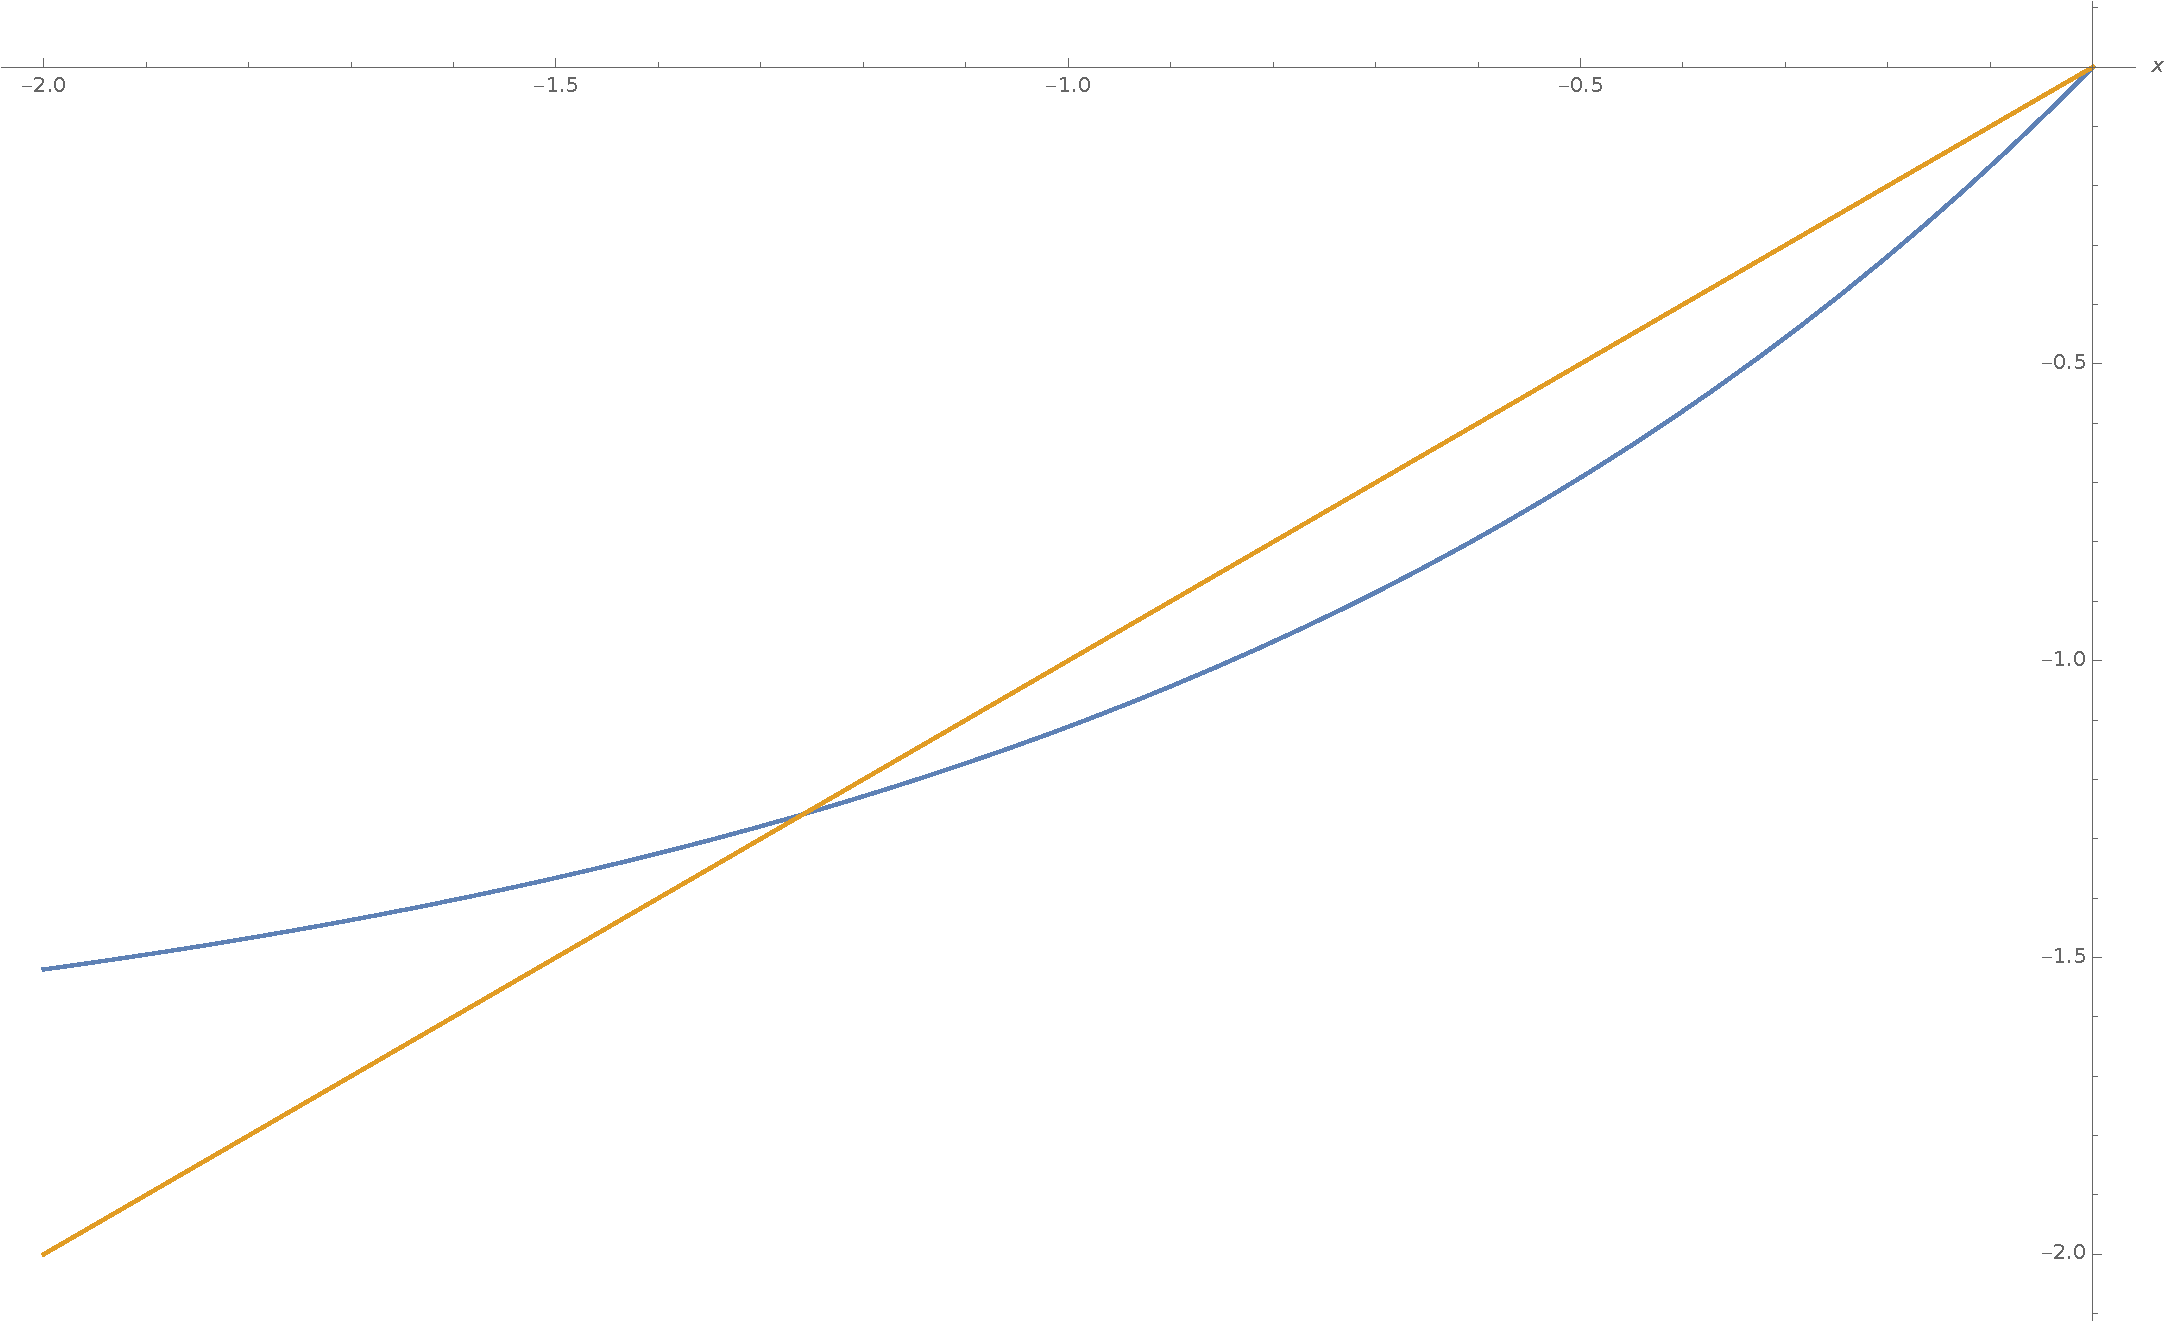
\includegraphics[width=\textwidth]{SELU-negative-pushing.pdf}
\caption{Überhang der $\selu$-Funktion für betragsmäßig kleine dendritische Potentiale}
\end{figure}
\end{enumerate}
\end{enumerate}
\item
\begin{enumerate}[label=\roman*)]
\item Vergleich der verschiedenen Transferfunktionen in der Anwendung:
\begin{figure}[H]
\centering
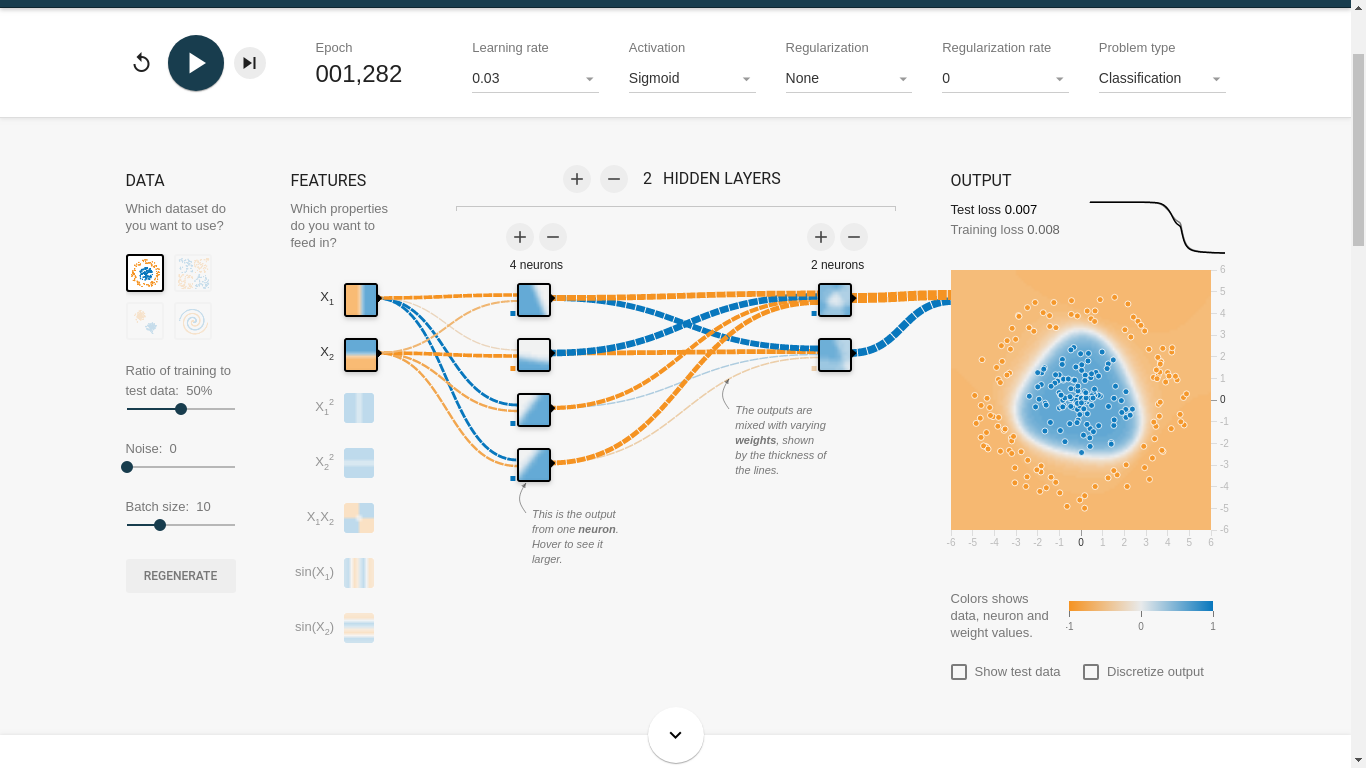
\includegraphics[width=\textwidth]{sigmoid.png}
\caption{Transferfunktion $\sig$}
\end{figure}
\begin{figure}[H]
\centering
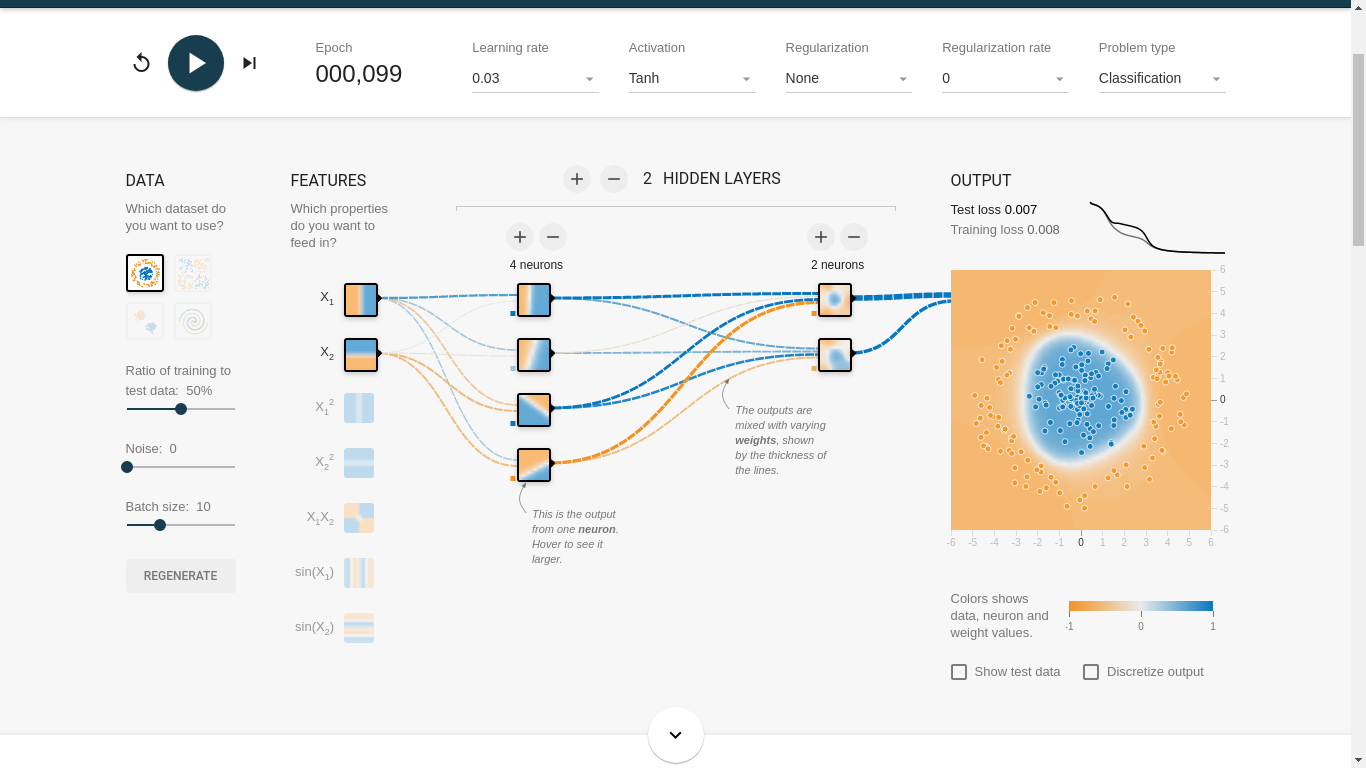
\includegraphics[width=\textwidth]{tanh.png}
\caption{Transferfunktion $\tanh(x)$}
\end{figure}
\begin{figure}[H]
\centering
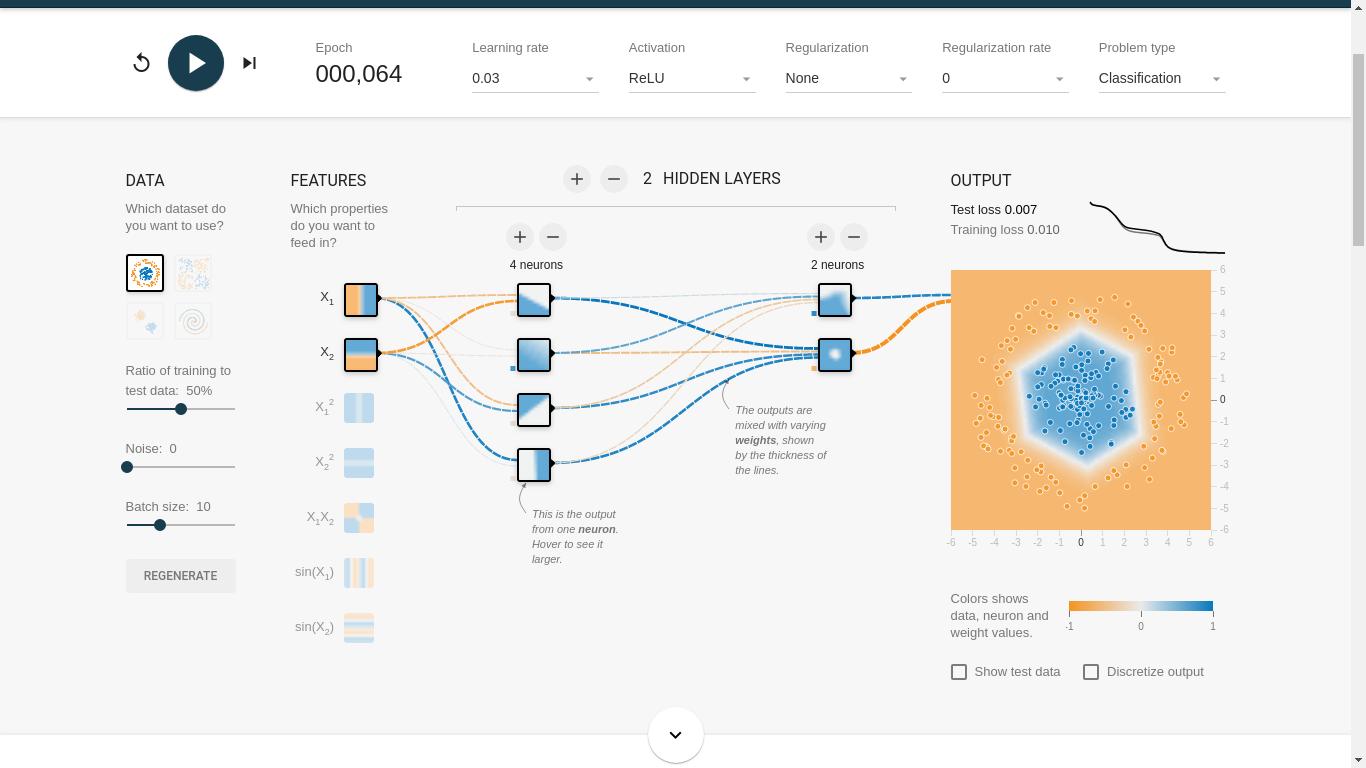
\includegraphics[width=\textwidth]{ReLU.png}
\caption{Transferfunktion $\relu$}
\end{figure}
\item In folgendem Beispiel leiden in der vorletzten Schicht das erste und dritte Neuron unter dem Effekt von \textit{dying}$\relu$. Dadurch, dass die Beiden Neuronen kurz hinter der Ausgabeschicht liegen, kommt auch der Lernvorgang in den vorhergehenden Schichten durch diesen Effekt zum erliegen. Das lässt sich auch an dem nahezu konstanten Fehler in der Ausgabeschicht beobachten.
\begin{figure}[H]
\centering
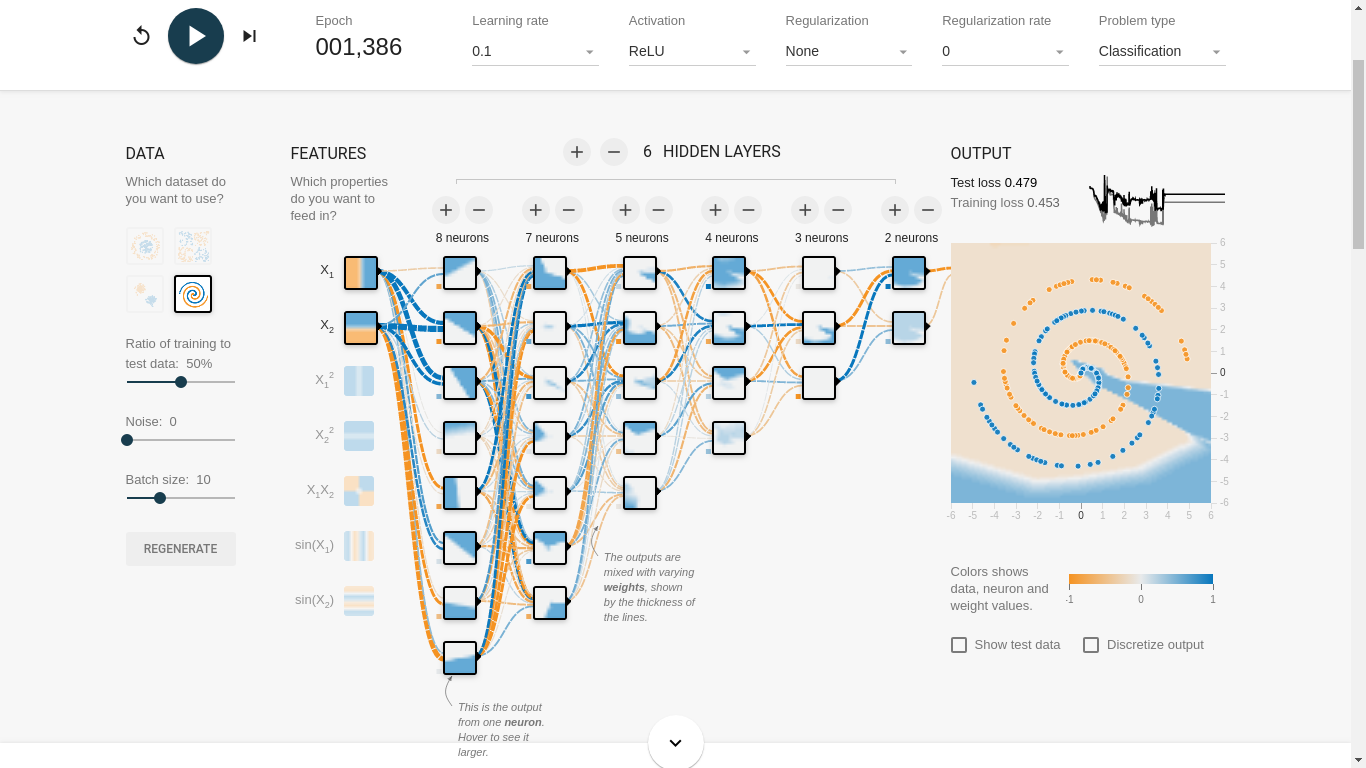
\includegraphics[width=\textwidth]{dyingReLU-complex-network.png}
\caption{Dying $\relu$ in einem komplexeren Netzwerk}
\end{figure}
\end{enumerate}

\item
  \begin{enumerate}[label=\alph*)]
  \item
    \begin{enumerate}[label=\roman*.]
      \item Bei der SELU Aktivierungsfunktion ist deutlich zu erkennen, dass die Standardabweichung der Aktivierungen für tiefere Schichten gegen 1 geht. Für den Gradienten ist zu erkennen, dass der Mittelwert während der Rückwärtsphase gegen 0 geht.
      \item Die Asymetrie der ReLU und ELU Funktionen ist am Stärksten bei den Aktivierungen der ersten Schichten ersichtlich. Besonders bei ReLU ist nicht nur der Mittelwert stark von 0 verschieden, auch der Wertebereich ist stark asymetrisch.
      \item Die Aktivierungen liegen in dem Bereich, in dem die Ableitung von $\tanh$ noch nicht gegen 0 geht.
      \item Die SELU Transferfunktion weist die größten Gradienten auf, folglich wird mit dieser Funktion am meisten gelernt.
    \end{enumerate}
  \item 3D Plot
  \begin{itemize}
\item[tanh] Die Verteilung wird bei tieferen Schichten zunehmend schmaler, da die Funktionswerte des $\tanh$ zwischen 0 und 1 liegen, und die Funktionswerte von diesen Werten in immer kleinerem Wertebereich liegen.
\item[ReLU] Die Verteilung wird noch schmaler als bei $\tanh$, da viele der Eingabewerte ($u<0$) direkt auf 0 abgebildet werden.
\item[ELU] Auch hier treten die gleichen Effekte wie bei $\tanh$ und ReLU auf, zusätzlich ist besonders bis ca. Layer 10 die Asymetrie der Transferfunktion in der Verteilung zu erkennen.
\item[SELU] Hier werden die oben betrachteten normalisierenden Eigenschaften der SELU Funktion ersichtlich: Die Verteilung bleibt über die Layer hinweg breit und konzentriert sich nicht um 0.
\end{itemize}
  \end{enumerate}

\end{enumerate}
\end{document}
